\documentclass[resume]{subfiles}


\begin{document}
\section{Modèles dynamiques}
\begin{figure}[H]
\centering
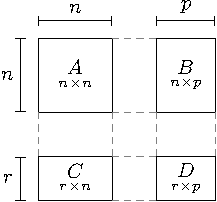
\includegraphics[scale=1.5]{drwg_0.pdf}
\end{figure}
\subsection{Rétroaction positive}

\begin{figure}[H]
    \centering
    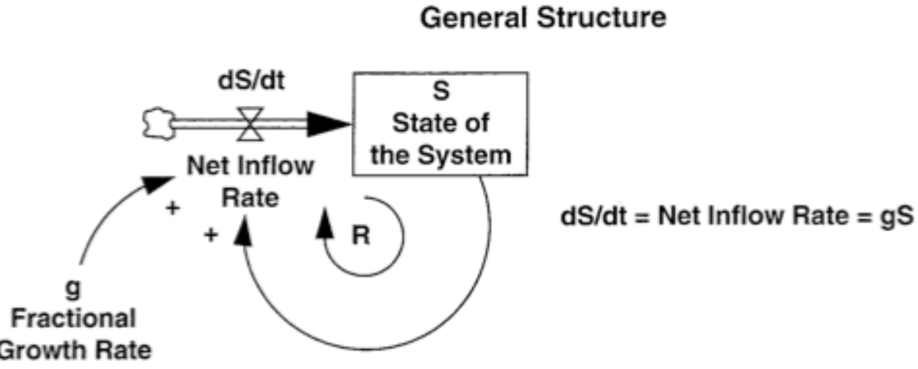
\includegraphics[width=1\columnwidth]{Figures/FDM_1.png}
\end{figure}

Le stock accumule du inflow $S(t)=S(0)e^{gt}$ 

Le temps de doublement du stock est de $2S(0)=S(0)e^{gt_d}$ on a donc $t_d=\frac{ln(2)}{g}=\frac{70}{100g}$

\subsection{Rétroaction négative et décroissance exponentielle}

\begin{figure}[H]
    \centering
    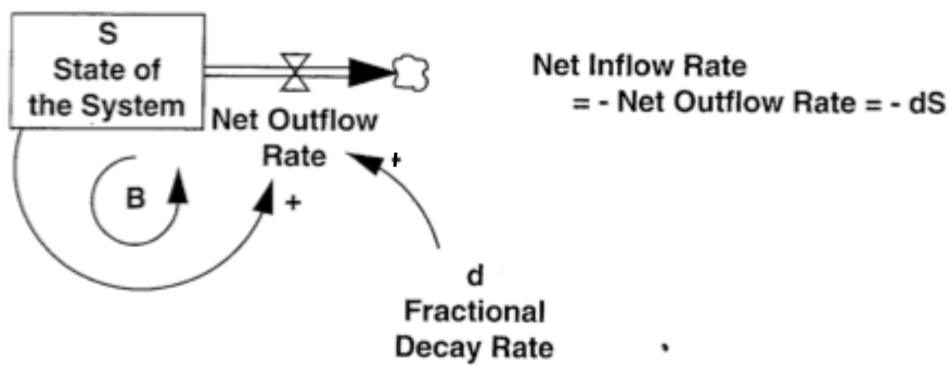
\includegraphics[width=1\columnwidth]{Figures/FDM_2.png}
\end{figure}

Le stock perd du outflow $S(t)=S(0)e^{-dt}$ 

Le temps de division par 2 du stock est de $t_d=ln(2)\tau=0.70\tau$ 

\subsection{Système non linéaires croissance en S}

\begin{figure}[H]
    \centering
    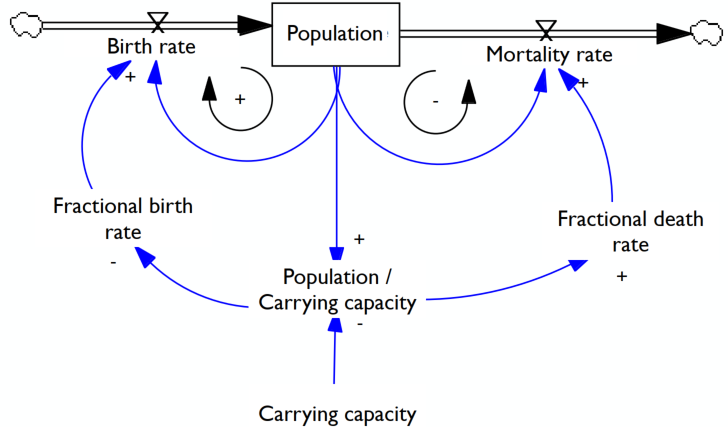
\includegraphics[width=1\columnwidth]{Figures/FDM_3.png}
\end{figure}

L'équation du système est
$$\frac{dP}{dt}=b(\frac{P}{C})P-d(\frac{P}{C})P$$

La croissance nette est une fonction de la population P :
$$\frac{dP}{dt}=g(P,C)P=g(1-\frac{P}{C})P$$


\subsection{Modèle logistique}
\begin{itemize}
\item $P$ : Population
\item $C$ : Capacité (carrying capacity)
\item $P_0$ : Population initiale
\item $g$ : gain
\end{itemize}
$$\frac{dP}{dt}=g(1-\frac{P}{C})$$
Solution de l'équation 
$$P(t)= \frac{C}{1+[\frac{C}{P_0}-1]e^{-gt}}$$

\subsection{Modèle SI et SIR}
\begin{itemize}
\item $S$ : susceptibles
\item $I$ : infectés
\item $R$ : rétablit
\item $I_R$ : Infection Rate
\item $R_R$ : recovery rate
\item $c$ : taux de contact
\item $i$ : taux d'infectiosité
\item $d$ : durée moyenne de maladie
\end{itemize}

\begin{figure}[H]
    \centering
    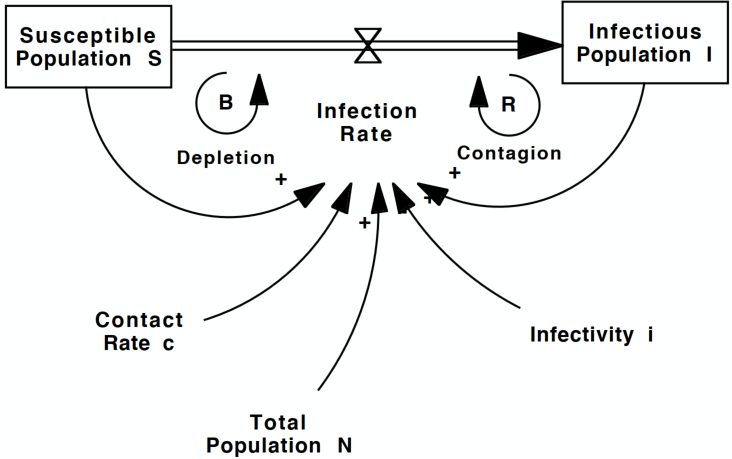
\includegraphics[width=1\columnwidth]{Figures/SI_1.png}
\end{figure}

\subsubsection{Equation du modèle SI}
$$N=S+I \rightarrow \frac{dS}{dt}=-(ciS)\frac{I}{N}= -(I_R)$$
$$\frac{dI}{dt}=ci\cdot I(1-\frac{I}{N})$$

\begin{figure}[H]
    \centering
    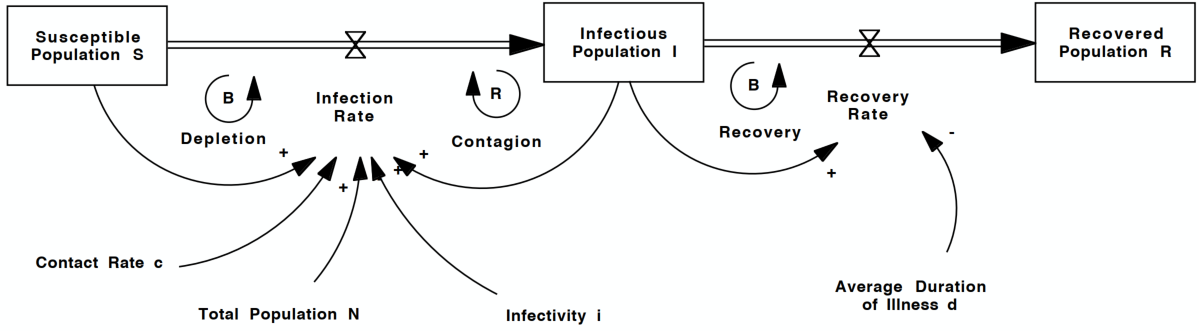
\includegraphics[width=1\columnwidth]{Figures/SIR_1.png}
\end{figure}

\subsubsection{Equation du modèle SIR}

\begin{align*}
\frac{dS}{dt}&=-(c\cdot i\cdot S)\frac{I}{N}\\
\frac{dR}{dt}&=R_R =\frac{I}{d}\\
\frac{dI}{dt} &= I_R=(c\cdot i\cdot S)\frac{I}{N}-\frac{I}{d}\\
N&=S+I+R
\end{align*}


Point de bascule
$$I_R > R_R \rightarrow c\cdot i\cdot S(\frac{I}{N}) > \frac{I}{d}$$
ou
$$c\cdot i\cdot d(\frac{S}{N} > 1)$$

\subsection{Retard}

Un retard est un processus dont la sortie correspond à l’entrée translatée dans le temps

\begin{figure}[H]
\centering
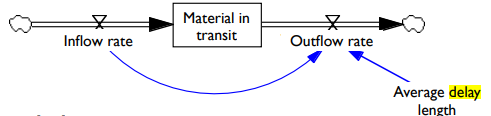
\includegraphics[width=6.00cm]{img_24.png}
\end{figure}

\end{document}